\documentclass[12pt,twoside,a4paper]{article} 

\usepackage{color,amssymb,amsmath,mathtools} 
\usepackage{fullpage,caption, listings,clrscode,placeins}
\usepackage{amsmath,bm}
\usepackage{subfig}
\usepackage{float}
% \usepackage{graphicx}
 
 % Metadata info
\newcommand{\mytitle}{Project 1} 
\newcommand{\mydate}{\today} 
\newcommand{\myauthors}{Prameth Gaddale}

% Setting Hyperref parameters
\usepackage[
	bookmarks,
	bookmarksnumbered,
	pdfpagemode={UseOutlines},
	plainpages=false,
	pdfpagelabels=true,
	pdfauthor={\myauthors},
	pdftitle={\mytitle},
	pagebackref=true,
	pdftex,
	colorlinks=true,
	linkcolor=red,
	urlcolor={blue}, 
	pagebackref=true]
	{hyperref}

\title{\mytitle}
\author{\myauthors}
\date{\mydate}

% Some useful commands from CVPR
\usepackage{xspace}
\makeatletter
\DeclareRobustCommand\onedot{\futurelet\@let@token\@onedot}
\def\@onedot{\ifx\@let@token.\else.\null\fi\xspace}
\def\eg{\emph{e.g}\onedot} \def\Eg{\emph{E.g}\onedot}
\def\ie{\emph{i.e}\onedot} \def\Ie{\emph{I.e}\onedot}
\def\cf{\emph{c.f}\onedot} \def\Cf{\emph{C.f}\onedot}
\def\etc{\emph{etc}\onedot} \def\vs{\emph{vs}\onedot}
\def\wrt{w.r.t\onedot} \def\dof{d.o.f\onedot}
\def\etal{\emph{et~al}\onedot}
\makeatother


\pagestyle{empty}
\usepackage{fancyref,fancyhdr}
%\usepackage[hmarginratio=1:1, top=2.0cm, bottom=5.0cm, left=1cm, right=1cm]{geometry}
\setlength{\headheight}{14pt}
\setlength{\headsep}{15pt}
\setlength{\footskip}{50pt}
\pagestyle{fancy}
\fancyhf{}
\fancyhf[HLE,HRO]{\footnotesize{\myauthors}}
\fancyhf[HLO,HRE]{\footnotesize{\mydate}}
\fancyhf[FLO,FRE]{\footnotesize{\mytitle}} 
\fancyhf[FLE,FRO]{\thepage }


\usepackage[pdftex]{graphicx}
\DeclareGraphicsExtensions{.pdf,.png,.jpg,.eps}

% 
\usepackage[numbers, sort&compress]{natbib}

\usepackage[senames,dvipsnames,svgnames,table]{xcolor}

\newenvironment{tightitemize} % Defines the tightitemize environment which modifies the itemize environment to be more compact
{\vspace{-\topsep}\begin{itemize}\itemsep1pt \parskip0pt \parsep0pt}
{\end{itemize}\vspace{-\topsep}} 

% If you want to write proofs
\newtheorem{claim}{Claim}[section]
\newtheorem{lemma}{Lemma}[section]

% Some useful packages (look at booktabs for good looking tables)
\usepackage{subcaption,booktabs,placeins}

%BEGIN THE DOCUMENT

\begin{document}
\maketitle

\begin{abstract}

In this day and age, automation is crucial in various industries which involve laborious and repetitive tasks. This project covers regression and classification problems, which are considered to be one of basic techniques of \textit{Pattern Recognition}. I've implemented linear models for regression, along with methods to optimize the parameters/weights of these models through the use of \textit{Maximum Likelihood Estimation} and \textit{Maximum A Posteriori Estimation}. Additonally, for classification models I've implemented the Fisher projection algorithm for the \textit{Taiji} dataset. I've also introduced the key aspects of the \textit{Central Limit Theorem}, in addition to answering few questions regarding estimating probability distributions.

\end{abstract}
\vspace{1ex}

\tableofcontents
% Break until the next page
\vfill
\pagebreak

% SECTIONS

\section{Linear Regression}

Supervised learning problems with the training data comprising of input vectors along with their corresponding target vectors, and the desired output consisting of one or more continuous variables is called \textit{Regression}. Bishop\cite{ChrisPRML} mentions about the use of polynomial curve fitting as an example to illustrate the usage and role of linear regression in real-world problems.\\
In polynomial curve fitting, we are given a training set (of $N$ examples) of $\textbf{x}$, where $\textbf{x} \equiv (x_1,...,x_N)^T$ and their corresponding target values $\textbf{t} \equiv (t_1,...,t_N)^T$.\\
Primarily, the objective of polynomial curve fitting is to find relevant parameters(represented by polynomial coefficients) $w_0, w_1, ... w_M$ that fit a polynomial function of degree $M$ represented as \ref{POLY},

\begin{equation}\label{POLY}
    y(x, \textbf{w}) = w_0 + w_1x + w2+w^2 + ... + w_Mx^M = \sum_{j=0}^{M}w_jx^j
\end{equation}
To arrive to our objective, we have to parameters that satisfy the minimization of an \textit{error function}, that measures the magnitude of misfit between our targets and predictions. \\ 
A suitable criteria for optimizing the model parameters is to minimize the squared sum between the targets and predicted values, mentioned in \ref{ERRML1}.
\begin{equation}\label{ERRML1}
    E(\textbf{w}) = \frac{1}{2}\sum_{n=1}^{N}\{y(x^n, \textbf{w})-t_n\}^2
\end{equation}
The two most popular approaches to solve the error function and estimate the model parameters which take the uncertainty into consideration through the use of Bayesian statistics \cite{statistical} are:
\begin{enumerate}
    \item Maximum Likelihood Estimator
    \item Maximum A Posteriori Estimator
\end{enumerate}
%-------------------------------------------------------------------------
\subsection{Maximum Likelihood Estimator}
In Maximum Likelihood Estimation, the main assumption is that the ground truth values (represented by $t_i$) follow a Gaussian distribution. The assumed distribution is spread over with mean value represented by the model prediction values, and the variance matrix (for multivariate datasets) as shown in \eqref{1.60}.

\begin{equation}\label{1.60}
    p(t|x,\textbf{w}, \beta) = \mathcal{N}(t|y(x,\textbf(w)),\beta^{-1})
\end{equation}
However, for a multivariate Gaussian distribution if we apply the i.i.d criterion which states that each example sampled from the dataset is independent and identically distributed we can write the joint conditional probability distribution in the product-form as \eqref{1.61}
\begin{equation}\label{1.61}
    p(t|x,\textbf{w}, \beta) = \prod_{n=1}^{N}\mathcal{N}(t|y(x,\textbf(w)),\beta^{-1})
\end{equation}
We also know that the standard Gaussian distribution is represented by \eqref{1.46},
\begin{equation} \label{1.46}
    \mathcal{N}(x|\mu,\sigma^2) = \frac{1}{(2\pi\sigma^2)^{1/2}}\exp\{-\frac{1}{2\sigma^2}(x-\mu)^2\}
\end{equation}
Now taking the equation \eqref{1.61}, applying the general equation \eqref{1.46} and taking the natural-logarithm across both the sides, we get,
\begin{align} \label{1.62}
\ln p(t|x,\textbf{w}, \beta) =& \sum_{n=1}^{N} \ln \{ \mathcal{N}(t_n|y(x_n,\textbf{w}),\beta^{-1}) \} \\
=& \sum_{n=1}^{N} \ln \{ \frac{1}{(2\pi\beta^{-1})^{1/2}}\exp\{-\frac{1}{2\beta^{-1}}\{t_n-y(x_n,\textbf{w})\}^2\}\} \\
=&\sum_{n=1}^{N} \ln \{ \frac{1}{(2\pi\beta^{-1})^{1/2}} \} + \sum_{n=1}^{N} \ln \{\exp\{-\frac{1}{2\beta^{-1}}\{t_n-y(x_n,\textbf{w})\}^2\}\} \\
=& N\ln \{ \frac{\beta}{(2\pi)} \}^{1/2} + \sum_{n=1}^{N} {-\frac{\beta}{2}\{y(x_n,\textbf{w})-t_n\}^2} \\
\ln p(t|x,\textbf{w}, \beta) =& -\frac{\beta}{2}\sum_{n=1}^{N} {\{y(x_n,\textbf{w})-t_n\}^2} + \frac{N}{2}\ln\beta - \frac{N}{2}\ln(2\pi) \label{LOGLL}
\end{align}
From statistics \cite{statistical}, we know that \eqref{LOGLL} is represented as log-likelihood and the first term on the right-hand-side, $-\frac{\beta}{2}\sum_{n=1}^{N} {\{y(x_n,\textbf{w})-t_n\}^2}$ resembles the \textit{\textbf{sum of the squared error}}. Hence, maximizing the log-likelihood function is equivalent to minimizing the negative log-likelihood function. \\
Taking negative on both sides, we get the equation of negative log-likelihood which is used to 
\begin{equation} \label{NLL}
    -\ln p(t|x,\textbf{w}, \beta) = \frac{\beta}{2}\sum_{n=1}^{N} {\{y(x_n,\textbf{w})-t_n\}^2} - \frac{N}{2}\ln\beta + \frac{N}{2}\ln(2\pi)
\end{equation}
We can represent the error function of \textit{Maximum Likelihood Estimator} by \eqref{ERRML2}
\begin{equation}\label{ERRML2}
    E_{ML}(\textbf{w}) = \frac{\beta}{2}\sum_{n=1}^{N} {\{y(x_n,\textbf{w})-t_n\}^2} - \frac{N}{2}\ln\beta + \frac{N}{2}\ln(2\pi)
\end{equation}
One of the fundamental operation to find critical points of a function with respect to a specific parameter is to equate the partial derivative of the function to zero and solving for the parameter. Applying that strategy to equation \eqref{ERRML2} with respect to \textbf{w} we get,
\begin{align}
\frac{\partial E_{ML}(\textbf{w})}{\partial \textbf{w}} =& 0\\
\frac{\partial}{\partial \textbf{w*}} \left( \frac{\beta}{2}\sum_{n=1}^{N} {\{y(x_n,\textbf{w})-t_n\}^2} - \frac{N}{2}\ln\beta + \frac{N}{2}\ln(2\pi) \right ) =& 0 \\
\frac{1}{2}.2.\sum_{n=1}^{N}\frac{\partial y_n}{\partial \textbf{w}_i}(y_n-t_n) =& 0 \\
\sum_{n=1}^{N}\frac{\partial y_n}{\partial \textbf{w}_i}(\sum_{j=0}^{M}{w_jx^j_n}-t_n) =& 0 \\
\sum_{n=1}^{N}x_n^i(\sum_{j=0}^{M}{w_jx^j_n}-t_n) =& 0 \\
\sum_{n=1}^{N}x_n^i\sum_{j=0}^{M}{w_jx^j_n} - \sum_{n=1}^{N}x_n^it_n =& 0 \\
\sum_{n=1}^{N}\sum_{j=0}^{M}{x_n^iw_jx^j_n} - \sum_{n=1}^{N}x_n^it_n =& 0 \\
\sum_{n=1}^{N}\sum_{j=0}^{M}{x^{i+j}_nw_j} - \sum_{n=1}^{N}x_n^it_n =& 0 \label{MLDERSUM}
\end{align}
Converting the result from the summation-scalar format present in \eqref{MLDERSUM} to matrix-format we get,
\begin{align}
\textbf{X}^T\textbf{X}\textbf{w}_{ML} - \textbf{X}^Tt =& 0 \\
\textbf{X}^T\textbf{X}\textbf{w*}_{ML} =& \textbf{X}^Tt \\
\textbf{w}_{ML} =& (\textbf{X}^T\textbf{X})^{-1}\textbf{X}^Tt \label{WMLFINAL}
\end{align}
Where, \eqref{WMLFINAL} represents the optimal weights for the polynomial with respect to minimizing the negative log-likelihood.\\
We can find the predictions of the model function by applying,
\begin{equation} \label{MLPRED}
    \textbf{y} = \textbf{w}^T_{ML}\textbf{X}
\end{equation}
\subsubsection*{Design Matrix Input}
However, in real-life situations the input is in the form of multiple dimensions and is a function of the input vector either through pre-processing steps or through the use of higher dimensional polynomial for the model fit. In that case we can consider the design matrix in the form of $\phi(x_n)$ and modify our objective function as,
 \begin{equation}
     \triangledown\ln p(t|w,\beta) = \triangledown \left( \sum_{n=1}^{N}\{t_n - \textbf{w}^T\phi(x_n)\}^2 \right)
 \end{equation}
Applying partial derivative with respect to \textbf{w} and solving for \textbf{w*} we get

\begin{align}
\frac{\partial E_ML(\textbf{w})}{\partial \textbf{w*}} =& 0\\
\frac{\partial}{\partial \textbf{w*}} \{ \frac{1}{2}\sum_{n=1}^{N}\{t_n - \textbf{w}^T\phi(x_n)\}^2 \} =& 0 \\
\sum_{n=1}^{N}t_n\phi(x_n)^T - \textbf{w}^T\left(\sum_{n=1}^{N}{\phi(x_n)\phi(x_n)^T} \right) =& 0 \\
\textbf{w}^T\left(\sum_{n=1}^{N}{\phi(x_n)\phi(x_n)^T} \right) =& \sum_{n=1}^{N}t_n\phi(x_n)^T \\
\textbf{w}^T(\Phi\Phi^T) =&\textbf{t}\Phi^T \\
\textbf{w}^T =& (\Phi\Phi^T)^{-1}\textbf{t}\Phi^T \\
\textbf{w}_{ML} =& (\Phi^T\Phi)^{-1}\Phi^T\textbf{t} \label{WML}
\end{align}
Hence we can find the predictions of the model function by applying,
\begin{equation} \label{MLPRED2}
    y = \textbf{w}^T\phi(x_n)
\end{equation}
Similarly, we can find the optimal value of the parameter $\beta$ by \eqref{BETAML},
\begin{equation} \label{BETAML}
    \beta_{ML}^{-1} = \frac{1}{N}\sum_{n=1}^{N}\{t_n - \textbf{w}_{ML}^T\phi(x_n)\}^2
\end{equation}
Hence, the distribution represented by the Gaussian distribution assumption gets converted through the use of optimal values as,
\begin{equation} \label{PREDDML}
    p(t|x,\textbf{w}_{ML},\beta_{ML}) = \mathcal{N}(y(x,\textbf{w}_{ML}), \beta^{-1}_{ML})
\end{equation}

%-------------------------------------------------------------------------
\pagebreak
\subsection{Maximum A Posteriori Estimator}
Unlike \textit{Maximum Likelihood Estimation} where the posterior distribution on the ground truth was assumed to be from a Gaussian distribution, Maximum A Posteriori Estimator introduces a prior distribution on the weight vector \textbf{w}. That could be written mathematically as in \eqref{LN1}. Using the general Gaussian distribution equation and applying natural logarithm to \eqref{LNFINAL}.
\begin{align}
p(\textbf{w}|\alpha) =& \mathcal{N}(\textbf(w)|0,\alpha^{-1}\textbf{I}) \label{LN1}\\
=& \frac{1}{(2\pi\alpha^{-1})^{1/2}}\exp\{-\frac{1}{2\alpha^{-1}}(\textbf{w}-0)^2\} \\
p(\textbf{w}|\alpha) =& \left( \frac{\alpha}{2\pi}\right)^{(M+1)/2} \exp\left\{ -\frac{\alpha}{2}\textbf{w}^T\textbf{w}\right\} \\
\ln p(\textbf{w}|\alpha) =& \frac{(M+1)}{2}.\ln\left( \frac{\alpha}{2\pi}\right) - \left\{ \frac{\alpha}{2}\textbf{w}^T\textbf{w}\right\} \label{LNFINAL}
\end{align}
From probability theory we know that,
\begin{align}
Posterior \propto& \ Likelihood * Prior\\
    p(\textbf{w}|\textbf{x},\textbf{t},\alpha,\beta) \propto& p(\textbf{t}|\textbf{x},\textbf{w},\beta) p(\textbf{w}|\alpha) \\
    \ln p(\textbf{w}|\textbf{x},\textbf{t},\alpha,\beta) \propto& \ln p(\textbf{t}|\textbf{x},\textbf{w},\beta) + \ln p(\textbf{w}|\alpha) \\
    \ln p(\textbf{w}|\textbf{x},\textbf{t},\alpha,\beta) =& \ln p(\textbf{t}|\textbf{x},\textbf{w},\beta) + \ln p(\textbf{w}|\alpha) + constant \label{PLP}
\end{align}

Substituting the equations \eqref{LOGLL} and \eqref{LNFINAL} in \eqref{PLP} we get,

\begin{multline}
        \ln p(\textbf{w}|\textbf{x},\textbf{t},\alpha,\beta) = {\left( -\frac{\beta}{2}\sum_{n=1}^{N} {\{y(x_n,\textbf{w})-t_n\}^2} + \frac{N}{2}\ln\beta - \frac{N}{2}\ln(2\pi) \right )} \\ + \left ( \frac{(M+1)}{2}.\ln\left( \frac{\alpha}{2\pi}\right) - \left\{ \frac{\alpha}{2}\textbf{w}^T\textbf{w}\right\} \right ) + constant
\end{multline}

\begin{multline}
        \ln p(\textbf{w}|\textbf{x},\textbf{t},\alpha,\beta) = -\frac{\beta}{2}\sum_{n=1}^{N} {\{y(x_n,\textbf{w})-t_n\}^2} + \frac{N}{2}\ln\beta - \frac{N}{2}\ln(2\pi) \\ + \frac{(M+1)}{2}.\ln\left( \frac{\alpha}{2\pi}\right) - \left\{ \frac{\alpha}{2}\textbf{w}^T\textbf{w}\right\} + constant
\end{multline}

\begin{multline} \label{NLLMAP}
       - \ln p(\textbf{w}|\textbf{x},\textbf{t},\alpha,\beta) = \frac{\beta}{2}\sum_{n=1}^{N} {\{y(x_n,\textbf{w})-t_n\}^2} - \frac{N}{2}\ln\beta + \frac{N}{2}\ln(2\pi) \\ - \frac{(M+1)}{2}.\ln\left( \frac{\alpha}{2\pi}\right) + \left\{ \frac{\alpha}{2}\textbf{w}^T\textbf{w}\right\} + constant
\end{multline}

Ignoring the constants (for simplicity as they would be equate to zero on taking the partial derivative with respect to \textbf{w}) from \eqref{NLLMAP} we can find the maximum of the posterior by minimizing the following equation,
\begin{equation}
     - \ln p(\textbf{w}|\textbf{x},\textbf{t},\alpha,\beta) = \frac{\beta}{2}\sum_{n=1}^{N} {\{y(x_n,\textbf{w})-t_n\}^2} + \left\{ \frac{\alpha}{2}\textbf{w}^T\textbf{w}\right\} 
\end{equation}
\begin{align}
    \triangledown \left(- \ln p(\textbf{w}|\textbf{x},\textbf{t},\alpha,\beta) \right ) =& 0 \\
    \triangledown \left( \frac{\beta}{2}\sum_{n=1}^{N} {\{y(x_n,\textbf{w})-t_n\}^2} + \left\{ \frac{\alpha}{2}\textbf{w}^T\textbf{w}\right\}  \right ) =& 0 \\
    \triangledown \left( \frac{\beta}{2}\sum_{n=1}^{N} {\{ \textbf{w}^T\textbf{X}-t_n\}^2} + \left\{ \frac{\alpha}{2}\textbf{w}^T\textbf{w}\right\}  \right ) =& 0 \\
    2*\frac{\beta}{2}\left ( \sum_{n=1}^{N} {\{ \textbf{w}^T\textbf{X}-t_n\}^T\textbf{X}} \right) + \left\{ 2*\frac{\alpha}{2}\textbf{w}\right\} =& 0 \\
    \beta( \textbf{X}^T\textbf{X}\textbf{w}-\textbf{X}^T\textbf{t})+ \alpha\textbf{w} =& 0 \\
    \beta\textbf{X}^T\textbf{X}\textbf{w}-\beta\textbf{X}^T\textbf{t}+ \alpha\textbf{w} =& 0 \\
    \textbf{X}^T\textbf{X}\textbf{w}+ \frac{\alpha}{\beta}\textbf{w} =& \textbf{X}^T\textbf{t} \\
 \textbf{w} =& \left(\textbf{X}^T\textbf{X} + \frac{\alpha}{\beta}\textbf{I}\right)^{-1}\textbf{X}^T\textbf{t} \\
 \textbf{w}_{MAP} =& \left(\textbf{X}^T\textbf{X} + \lambda\textbf{I}\right)^{-1}\textbf{X}^T\textbf{t}
\end{align}
We can observe that, this optimization criterion is equivalent to minimizing the regularized sum-of-squares error, with the parameter $\lambda = \alpha/\beta$.

%-------------------------------------------------------------------------
\pagebreak
\subsection{Report}
\subsubsection{Dataset}
Given dataset (shown in \ref{fig: DATASET}) consists of input values($x$), ground truth values($y$), target values($t$) and random noise values($sigma$) added to ground truth values to produce targets.
\begin{figure}[H]
    \centering
    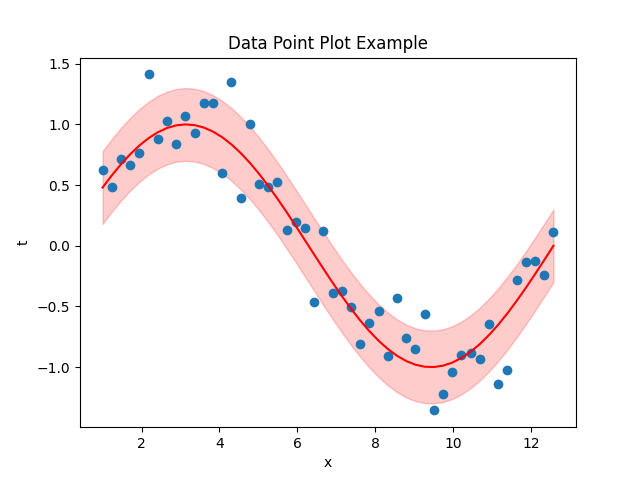
\includegraphics{results/gt_data.png}
    \caption{Given training dataset consists of ($x$), ($y$), ($t$) and($sigma$) values.}
    \label{fig: DATASET}
\end{figure}
\begin{itemize}
    \item The ground truth values of the curve represent the equation $y = sin(0.5*x)$.
    \item The target values of the dataset are formed by adding a Gaussian noise to the ground truth points.
    \item The shaded part in \ref{fig: DATASET} represents the Gaussian noise spanned over the ground truth.
    \item The given dataset has variable \textit{num\_points} that could be used to change the number of points used for the experiment.
    \item The generated datasamples are stored in \textit{.npz} format.
\end{itemize}
%-------------------------------------------------------------------------
\pagebreak
\subsubsection{Visualization}

\subsubsection*{Maximum Likelihood Estimation}
For the dataset with $50$ training data points, here are the results observed for the \textit{Maximum Likelihood Estimation} Model.
\begin{figure}[H]
    \centering
    \subfloat[Model Degree: $0$]{
      \includegraphics[width=0.55\linewidth]{results/50_ml_0.png}}
    \subfloat[Model Degree: $1$]{
      \includegraphics[width=0.55\linewidth]{results/50_ml_1.png}}
    \hspace{0mm}
    \subfloat[Model Degree: $3$]{
      \includegraphics[width=0.55\linewidth]{results/50_ml_3.png}}
    \subfloat[Model Degree: $9$]{
      \includegraphics[width=0.55\linewidth]{results/50_ml_9.png}}
    \hspace{0mm}
    \caption{Maximum Likelihood Estimation Model Prediction Visualization}
    \label{MLFIG}
\end{figure}

\pagebreak
\subsubsection*{Maximum A Posteriori Estimation}
For the dataset with $50$ training data points, here are the results observed for the \textit{Maximum A Posteriori Estimation} Model.
\begin{figure}[H]
    \centering
    \subfloat[Model Degree: $0$]{
      \includegraphics[width=0.55\linewidth]{results/50_map_0.png}}
    \subfloat[Model Degree: $1$]{
      \includegraphics[width=0.55\linewidth]{results/50_map_1.png}}
    \hspace{0mm}
    \subfloat[Model Degree: $3$]{
      \includegraphics[width=0.55\linewidth]{results/50_map_3.png}}
    \subfloat[Model Degree: $9$]{
      \includegraphics[width=0.55\linewidth]{results/50_map_9.png}}
    \hspace{0mm}
    \caption{Maximum A Posteriori Estimation Model Prediction Visualization}
    \label{MAPFIG}
\end{figure}

%-------------------------------------------------------------------------
\subsubsection{Comparison}
In \ref{COMP}, comparisons of the Maximum Likelihood Model and the Maximum A Posteriori Model are observed for varying model degrees corresponding to 50 data points.
\begin{figure}[H]
    \centering
    \subfloat[Model Degree: $0$]{
      \includegraphics[width=0.5\linewidth]{results/50_ml_vs_map0.png}}
    \subfloat[Model Degree: $1$]{
      \includegraphics[width=0.5\linewidth]{results/50_ml_vs_map1.png}}
    \hspace{0mm}
    \subfloat[Model Degree: $3$]{
      \includegraphics[width=0.5\linewidth]{results/50_ml_vs_map3.png}}
    \subfloat[Model Degree: $9$]{
      \includegraphics[width=0.5\linewidth]{results/50_ml_vs_map9.png}}
    \hspace{0mm}
    \subfloat[Model Degree: $15$]{
      \includegraphics[width=0.5\linewidth]{results/50_ml_vs_map15.png}}
    \subfloat[Model Degree: $20$]{
      \includegraphics[width=0.5\linewidth]{results/50_ml_vs_map20.png}}
    \hspace{0mm}
    \caption{Maximum A Posteriori Estimation Model Prediction Visualization}
    \label{COMP}
\end{figure}
%-------------------------------------------------------------------------
\pagebreak
\subsubsection{Summary}
\begin{itemize}
    \item Predictions of both the \textit{Maximum Likelihood Estimation} and \textit{Maximum A Posterirori} models have been made and plotted.
    \item From \ref{MLFIG}, we can observe the polynomial degrees 0 and 1 weren't good fits of the underlying ground truth curve. The polynomial function representing were lines, and weren't able to capture the data distribution accurately.
    \item However, in \ref{MLFIG} we know that polynomial with degree 3 was able to provide a good fit for the data distribution, being \textit{just right} for the data modelling. But on the other hand, the polynomial with degree 9 was over-fitting the ground truth curve, but was trying to go through most of the target data points.
    \item Similar behaviour is observed in the case of \textit{Maximum A Posteriori Estimation} model as shown in \ref{MAPFIG}.
    \item Higher the model degree, the model fits the noisy data pretty well. However, when it comes to degree 9 polynomial, it overfits to the examples and isn't able to generate a proper sine-like curve to capture the ground truth distribution.
    \item Hence, in this case as well, the model degree 3 performed most optimally in terms of fitting to the noisy data distribution.
    \item Similarly, we can observe the model based comparison based on the varying degrees as shown in \ref{COMP}. We can see that the MAP model has smoothed out the overfit-effects at higher order compared to ML model which tries to capture every datapoint in the target space.
    \item Hence, we can say that higher order degrees for polynomials have overfitted the noisy training data, especially in the case of \textit{Maximum Likelihood Estimation}. However, \textit{Maximum A Posteriori Estimation} did a good job of smoothing out the noise at a certain extent without letting overfit the data distribution.
    \item This is because of the inherent regularization being applied by MAP model.
\end{itemize}

%-------------------------------------------------------------------------
\subsection{Extra Credit}
%-------------------------------------------------------------------------

\subsubsection{Additional Lambda Values}

The results for the regularized custom model with varying $\lnlambda$ values is shown in \ref{VARLN}. \\ We can observe that higher the value of regularization, the curve tends to become more linear and penalizes the weight vectors at a higher extent.

\begin{figure}[H]
    \centering
    \subfloat[Regularized Model $\ln \lambda = -13$]{
      \includegraphics[width=0.5\linewidth]{results/50_lnlambda-13.png}}
    \subfloat[Regularized Model $\ln \lambda = -15$]{
      \includegraphics[width=0.5\linewidth]{results/50_lnlambda-15.png}}
    \hspace{0mm}
    \subfloat[Regularized Model $\ln \lambda = -18$]{
      \includegraphics[width=0.5\linewidth]{results/50_lnlambda-18.png}}
    \subfloat[Regularized Model $\ln \lambda = 0$]{
      \includegraphics[width=0.5\linewidth]{results/50_lnlambda0.png}}
    \hspace{0mm}
    \subfloat[Regularized Model $\ln \lambda = 10$]{
      \includegraphics[width=0.5\linewidth]{results/50_lnlambda10.png}}
    \subfloat[Reguralized Model $\ln \lambda = 20$]{
      \includegraphics[width=0.5\linewidth]{results/50_lnlambda20.png}}
    \hspace{0mm}
    \caption{Additional lambda values model predictions}
    \label{VARLN}
\end{figure}
\begin{figure}[H]
    \centering
    \includegraphics[width=0.8\linewidth]{results/rmse-lnlambda.png}
    \caption{Root Mean Squared Error vs. $\ln \lambda$ plot.}
    \label{LNLAMBDARMSE}
\end{figure}
The plot \ref{LNLAMBDARMSE} represents the plot of Root Mean Squared Error vs $\ln\lambda$ values. For higher values of $\lnlambda$, models tends to underfit the training distribution and produces worse training error.
%-------------------------------------------------------------------------
\subsubsection{Varying Degree of Polynomial Order}
The table \ref{MLWEIGHTS} represents the weights of the Maximum Likelihood Model with varying degrees. 
\begin{table}[H]
\centering
\begin{tabular}{|c|c|c|c|c|c|c|}
\hline
\textbf{Weights}              & \textbf{M = 0} & \textbf{M = 1} & \textbf{M = 3} & \textbf{M = 6} & \textbf{M = 9} \\\hline
\textit{\textbf{$w_0^{ML}$}} & 0.009549       & 1.204800       & -0.185197      & -0.713196      & -1.367908      \\\hline
\textit{\textbf{$w_1^{ML}$}}  & -              & -0.176208      & 0.958219       & 1.860958       & 4.790468       \\\hline
\textit{\textbf{$w_2^{ML}$}} & - & - & -0.221176 & -0.794732 & -4.971345 \\\hline
\textit{\textbf{$w_3^{ML}$}} & - & - & 0.011743  & 0.184684  & 2.956968  \\\hline
\textit{\textbf{$w_4^{ML}$}} & - & - & -         & -0.026116 & -1.027571 \\\hline
\textit{\textbf{$w_5^{ML}$}} & - & - & -         & 0.001895  & 0.214036  \\\hline
\textit{\textbf{$w_6^{ML}$}} & - & - & -         & -0.000052 & -0.027113 \\\hline
\textit{\textbf{$w_7^{ML}$}} & - & - & -         & -         & 0.002043  \\\hline
\textit{\textbf{$w_8^{ML}$}} & - & - & -         & -         & -0.000084 \\\hline
\textit{\textbf{$w_9^{ML}$}} & - & - & -         & -         & 0.000001 \\\hline
\end{tabular}
\caption{Weights of the Maximum Likelihood model with varying degrees.}
\label{MLWEIGHTS}
\end{table}

The table \ref{MAPWEIGHTS} represents the weights of the Maximum A Posteriori Model with varying degrees.
\begin{itemize}
    \item We observe that Maximum Likelihood estimation model weights are higher compared to MAP model weights.
    \item The higher order coefficient are nearly non-existent in the case of the MAP model.
\end{itemize}

\begin{table}[H]
\centering
\begin{tabular}{|c|c|c|c|c|c|}
\hline
\textbf{Weights}              & \textbf{M = 0} & \textbf{M = 1} & \textbf{M = 3} & \textbf{M = 6} & \textbf{M = 9} \\ \hline
\textit{\textbf{$w_0^{MAP}$}} & 0.009549       & 1.204745       & -0.184890      & -0.674439      & 0.263706       \\ \hline
\textit{\textbf{$w_1^{MAP}$}} & -              & -0.176201      & 0.958032       & 1.803124       & 0.875506       \\ \hline
\textit{\textbf{$w_2^{MAP}$}} & - & - & -0.221146 & -0.764588 & -1.278764 \\ \hline
\textit{\textbf{$w_3^{MAP}$}} & - & - & 0.011742  & 0.177347  & 1.131148  \\ \hline
\textit{\textbf{$w_4^{MAP}$}} & - & - & -         & -0.025209 & -0.497739 \\ \hline
\textit{\textbf{$w_5^{MAP}$}} & - & - & -         & 0.001839  & 0.119170  \\ \hline
\textit{\textbf{$w_6^{MAP}$}} & - & - & -         & -0.000051 & -0.016513 \\ \hline
\textit{\textbf{$w_7^{MAP}$}} & - & - & -         & -         & 0.001324  \\ \hline
\textit{\textbf{$w_8^{MAP}$}} & - & - & -         & -         & -0.000057 \\ \hline
\textit{\textbf{$w_9^{MAP}$}} & - & - & -         & -         & 0.000001  \\ \hline
\end{tabular}
\caption{Weights of the Maximum A Posteriori model with varying degrees.}
\label{MAPWEIGHTS}
\end{table}


%-------------------------------------------------------------------------
\subsubsection{Varying Number of Sample Points}
Higher the data points used for fitting the polynomial, the model is able to perform better on capturing the underlying ground truth curve as shown in \ref{DATAP}.

\begin{figure}[H]
    \centering
    \subfloat[ML Model, 20 Data Points]{
      \includegraphics[width=0.5\linewidth]{results/20_ml_9.png}}
    \subfloat[MAP Model, 20 Data Points]{
      \includegraphics[width=0.5\linewidth]{results/20_map_9.png}}
    \hspace{0mm}
    \subfloat[ML Model, 200 Data Points]{
      \includegraphics[width=0.5\linewidth]{results/200_ml_9.png}}
    \subfloat[MAP Model, 200 Data Points]{
      \includegraphics[width=0.5\linewidth]{results/200_map_9.png}}
    \hspace{0mm}
    \caption{Maximum Likelihood and Maximum A Posteriori Estimation Model Prediction with varying data points.}
    \label{DATAP}
\end{figure}

%-------------------------------------------------------------------------
\subsubsection{Curse of Dimensionality}

%-------------------------------------------------------------------------
\pagebreak
\section{Classification}
Unlike regression problems, the objective of classification models is to assign input vector $\textbf{x}$ to one of \textit{K} discrete classes where $k = 1,...,K$. The \textit{decision regions} or \textit{decision boundaries} therefore represent the division of the input space, which are used to classify each input into disjoint classes.\\
\textit{Fisher Linear Discriminant Analysis} is considered to be a part of the family of linear models used for classification, where the decision boundaries are linear functions of the provided input vector $\textbf{x}$.
%-------------------------------------------------------------------------
\subsection{Fisher Projection}
In \textit{Fisher Linear Discriminant}, the algorithm tries to project the data from a high-dimensional space to a lower-dimensional space. However, inherently due to drop of dimensions, some of the key information is lost. The main goal of the algorithms is to find a \textbf{projection to a decision subspace that maximizes the \textit{class separation}}.
In Fisher projection, concurrently 2 operations are performed which could be considered as our objective function,
\begin{itemize}
    \item \textbf{Maximizing the distance between projected inter-class means.}
    \item \textbf{Minimizing the distance between projected intra-class variances.}
\end{itemize}
However, optimizing those functions individually is not possible. Hence, the goal is defined to maximize their ratio. They are mathematically viewed as following, \\
We tend to construct a Fisher project matrix \textbf{W} which aids int he transformation of the input data \textbf{x} as shown in \eqref{FPM}.
\begin{equation}\label{FPM}
    \textbf{y} = \textbf{W}^T\textbf{x}
\end{equation}
Applying the intra-class variance over all the given K classes, we get \eqref{SW}
\begin{equation}\label{SW}
    \textbf{S}_W = \sum_{k=1}^K\textbf{S}_k
\end{equation}
where of each class, the matrix $\textbf{S}_k$ is represented by,
\begin{equation}
    \textbf{S}_k = \sum_{n\in\textit{C}_k}(x_n - \textbf{m}_k)(x_n - \textbf{m}_k)^T
\end{equation}
If we have only two classes we get,
\begin{equation}
    \textbf{m}_1 = \frac{1}{N_1}\sum_{n\in\textit{C}_1}x_n,\qquad \textbf{m}_2 = \frac{1}{N_2}\sum_{n\in\textit{C}_2}x_n
\end{equation}
For multiple classes we have, 
\begin{equation}
    \textbf{m}_k = \frac{1}{N_k}\sum_{n\in\textit{C}_k}\textbf{x}_n
\end{equation}
The global mean of the given data is given by,
\begin{equation}\label{GLOBALM}
    \textbf{m} = \frac{1}{N}\sum_{k=1}^K N_k\textbf{m}_k
\end{equation}
Where the term $N = \sum_kN_k$ represented the total number of data points.
And the matrices $\textbf{S}_T$ and $\textbf{S}_B$ that aid in the construction of the projection matrix are given by, 
\begin{equation} \label{ST}
    \textbf{S}_T = \sum_{n=1}^N(\textbf{x}_n - \textbf{m})(\textbf{x}_n - \textbf{m})^T
\end{equation}

\begin{equation} \label{SB}
    \textbf{S}_B = \sum_{n=1}^N N_K(\textbf{m}_k - \textbf{m})(\textbf{m}_k - \textbf{m})^T
\end{equation}
Now, to find the most optimal \textbf{W} we find a criterion to minimize using the equations \eqref{ST} and \eqref{SB} as,
\begin{equation}
    J(\textbf{W}) = Tr\left( (\textbf{W}\textbf{S}_W\textbf{W}^T)^{-1} (\textbf{W}\textbf{S}_B\textbf{W}^T) \right )
\end{equation}
Minimizing this criterion, $J(w)$ is done by finding the eigen-vectors of $W = S_W^{-1}S_B$. \\
Hence, we can choose the eigenvectors that correspond to the $D'$ largest eigenvalues.

%-------------------------------------------------------------------------
\pagebreak
\subsection{Report}
%-------------------------------------------------------------------------
\subsubsection{Dataset}
Given dataset is of \textit{Taiji Poses} with 7 different poses and one transitional pose.
\begin{figure}[H]
    \centering
    \includegraphics{results/decision_boundary.png}
    \caption{Taiji Dataset Example Decision Boundary}
    \label{fig:my_label}
\end{figure}
%-------------------------------------------------------------------------
\subsubsection{Confusion Matrix}
\begin{figure}[H]
    \centering
    \subfloat[Taiji Training Data Confusion Matrix]{
      \includegraphics[width=0.6\linewidth]{results/taiji_train_confusion.png}}
    \hspace{0mm}
    \subfloat[Taiji Test Data Confusion Matrix]{
      \includegraphics[width=0.6\linewidth]{results/taiji_test_confusion.png}}
    \hspace{0mm}
    \caption{Taiji Training and Test Confusion Matrices}
\end{figure}
%-------------------------------------------------------------------------
\subsubsection{Classification Rates}
\begin{figure}[H]
    \centering
    \subfloat[Taiji Training Data Classification Rate Matrix]{
      \includegraphics[width=0.6\linewidth]{results/taiji_train_classification.png}}
    \hspace{0mm}
    \subfloat[Taiji Test Data Classification Rate Matrix]{
      \includegraphics[width=0.6\linewidth]{results/taiji_test_classification.png}}
    \hspace{0mm}
    \caption{Taiji Training and Test Classification Rate Matrices}
\end{figure}

\begin{table}[H]
\centering
\resizebox{\columnwidth}{!}{%
\begin{tabular}{|c|c|c|}
\hline
\textbf{Model} &
  \textbf{\begin{tabular}[c]{@{}c@{}}Overall Training \\ Classification Rate\end{tabular}} &
  \textbf{\begin{tabular}[c]{@{}c@{}}Overall Test \\ Classification Rate\end{tabular}} \\ \hline
LDA               & 0.95775 & 0.93451 \\ \hline
KNN: 3 Neighbors  & 0.98380 & 0.80224 \\ \hline
KNN: 5 Neighbors  & 0.97888 & 0.83231 \\ \hline
KNN: 7 Neighbors  & 0.97562 & 0.87156 \\ \hline
KNN: 10 Neighbors & 0.97324 & 0.88583 \\ \hline
\end{tabular}%
}
\caption{Overall Classification Rates of various classifiers, after performing Fisher projection.}
\label{OCRATE}
\end{table}

%-------------------------------------------------------------------------
\subsubsection{Analysis}

%-------------------------------------------------------------------------
\subsubsection{Conclusion}

%-------------------------------------------------------------------------
\subsection{Extra Credit}

%-------------------------------------------------------------------------
\pagebreak
\section{Central Limit Theorem}

%-------------------------------------------------------------------------
\subsection{Introduction}

According to Fischer \cite{CLT}, classical central limit theorem states that for a large enough sample size the population distribution can be assumed to be Gaussian. However, its essential to note that the sequence of random variables forming the population must be drawn from a distribution with finite mean and variance and must follow the i.i.d. criterion. \\
Bishop \cite{ChrisPRML}, mentions that the posterior distribution for a model is expected to become increasingly better approximated by a Gaussian distribution as the number of data points is increased.

Let us consider an unknown distribution with $n$ independent, identically distributed random variables $X_1, X_2, ..., X_n$, where is $n$ is very large with mean, $\mu$ and variance, $\sigma^2$. \\

Hence, we can find the mean, $\mu_N$ and variance, $\sigma^2_N$ as,
\begin{align}
\mu_N =& \frac{1}{n}(X_1+X_2+...+X_n) \\
      =& \frac{1}{n}(n*\mu) \\
\mu_N =& \mu
\end{align}

\begin{align}
\sigma^2_N =& Var\left( \frac{1}{n}(X_1+X_2+...+X_n) \right ) \\
           =& \left( \frac{1}{n} \right )^2 \left(Var(X_1)+Var(X_2)+...+Var(X_n) \right ) \\
           =& \left( \frac{1}{n} \right )^2 \left(\sigma^2+\sigma^2+...+\sigma^2 \right ) \\
           =& \left( \frac{1}{n} \right )^2(n\sigma^2) \\
\sigma^2_N =& \frac{\sigma^2}{n}
\end{align}

Hence, the approximate Gaussian distribution is formed with a mean, $\mu_N$ and variance, $\sigma^2_N$.
%-------------------------------------------------------------------------
\subsection{Question 1}

\subsubsection*{Question:}
\textbf{For a coin with a probability of heads of 0.6 in each flip, calculate the exact distribution of the total number of heads when the coin is flipped 5 times. Provide the equation(s) used to generate the result and a brief explanation of you reasoning.}

\subsubsection*{Solution:}
\label{Q1 Solution}
When a coin is flipped, there are two possible outcomes: head and tails each carrying a fixed probability. Given is coin is imbalanced in nature with the probability of head in each flip being \textbf{$0.6$}.\\
Binary outcome experiments such as coin-toss follow the \textbf{Binomial Distribution}. Let $X$ be the binomial random variable over the coin-toss experiment.\\
Hence, the probability mass function for the experiment representing the binomial random variable $X$ is given by,
\begin{equation} \label{BD1}
F(\mathbf{X = x}) = 
    \begin{cases}
        {{n}\choose{x}}p^{x}q^{n-x} & ,x = 0,1,2,...,n\\
        0   & ,otherwise
    \end{cases}
\end{equation}
The parameters in the binomial distribution are:
\begin{itemize}
    \item $n$: The total number of trials.
    \item $p$: The probability of success on a single trial.
    \item $q$: The probability of failure on a single trial.
    \item $x$: Represents the trial number(which is a whole number, $0\le x \le n$)
\end{itemize}
In our case, the probability of heads and tails adds up to 1. Hence we can write,
$$q=1-p$$
By incorporating that change in \eqref{BD1} we get,
\begin{equation} \label{BD2}
F(\mathbf{X = x}) = 
    \begin{cases}
        {{n}\choose{x}}p^{x}(1-p)^{n-x} & ,x = 0,1,2,...,n\\
        0   & ,otherwise
    \end{cases}
\end{equation}
We get $n=5$(as total number of coin flips is 5), $p=0.6$ and $q=0.4$.
\begin{equation} \label{BD3}
F(\mathbf{X = x}) = 
    \begin{cases}
        {{5}\choose{x}}(0.6)^{x}(0.4)^{5-x} & ,x = 0,1,2,...,n\\
        0   & ,otherwise
    \end{cases}
\end{equation}
Therefore \eqref{BD3} represents the probability distribution of total number of heads when the coin is flipped 5 times.\\
In short hand notation, we can also write that,
$$S_n \sim Binomial(n=5, p=0.6)$$
Hence, we can say that the exact distribution of the total number of heads if coin is flipped 5 times is represented by a Binomial Distribution with parameters $n=5$ and $p=0.6$.
%-------------------------------------------------------------------------
\subsection{Question 2}

\subsubsection*{Question:}
\textbf{Using the central limit theorem, approximate the distribution of the total number of heads when the coin is flipped 5000 times. Provide the equation(s) used to generate the result and a brief explanation of you reasoning.}

\subsubsection*{Solution:}
The coin-toss experiment as we know from \ref{Q1 Solution}, follows the Binomial Distribution for the probability estimation. However, for 5000 coin flips, calculation of probability through the use of factorials in the combination terms becomes a computationally expensive. From central limit theorem we know that, for a large number of trails in an experiment, we can approximate the population to be of a normal distribution. \\
\begin{itemize}
    \item Let $F_n$ represent the probability distribution we need to estimate for 5000 coin flips, which comes from a \textbf{Binomial Distribution}. $$F_n \sim Binomial(n, p)$$
    \item Let the approximate normal distribution have a mean, $\mu_N$ and variance $\sigma^2_N$.
    \item Let the approximate normal distribution have a mean, $\mu_N$ and variance $\sigma^2_N$.
\end{itemize}
From central limit theorem, we know that,
\begin{equation}\label{DMEAN}
    \mu_N = \mu
\end{equation}
\begin{equation}\label{DVAR}
    \sigma_N^2 = \frac{\sigma^2}{n}
\end{equation}

Some useful properties are:
\begin{itemize}
    \item \textbf{Mean}: $\mu = np$
    \item \textbf{Variance}: $\sigma^2 = np(1-p)$
\end{itemize}
For our case, we get,
$$F_{n = 5000} \sim Binomial(n = 5000, p = 0.6)$$
\begin{align*}
    Mean, \mu =& n*p \\
        =& 5000*0.6 \\
        \mu=& 3000
\end{align*}
\begin{align*}
    Variance, \sigma^2 =& n*p*(1-p) \\
        =& 5000*0.6*0.4 \\
        \mu=& 1200
\end{align*}
From \eqref{DMEAN} and \eqref{DVAR}, we get
$$\mu_N = 3000$$
\begin{align*}
    \sigma_N^2 =& \frac{\sigma^2}{n} \\
               =& \frac{1200}{5000}  \\
    \sigma_N^2 =& 0.24
\end{align*}
$$F_{n=5000} \sim Normal(\mu_N = 3000, \sigma^2_N = 0.24)$$
Hence, we can say that the exact distribution of the total number of heads if coin is flipped 5000 times can be approximated using Central Limit Theorem by a Gaussian Distribution with parameters $\mu_N = 3000$ and $\sigma^2_N = 0.24$.
%-------------------------------------------------------------------------

% BIBLIOGRAPHY
{\small
\bibliographystyle{IEEEtranN}
\bibliography{mybib}}

\end{document}
